\documentclass[11pt,a4paper]{article}

% ─────────────────────────────────────────────────────────────────────────────
%  Web Mining — TP1 : Clasificación de noticias de Página 12
%  Víctor Ruiz — Maestría en Ciencia de Datos — Universidad Austral
% ─────────────────────────────────────────────────────────────────────────────

\usepackage[utf8]{inputenc}
\usepackage[T1]{fontenc}
\usepackage[margin=2.4cm]{geometry}

% El paquete babel-spanish no está instalado en este equipo, así que en lugar de
% \usepackage[spanish]{babel} se renombran los rótulos manualmente (Tabla/Figura/
% Resumen/Apéndice). El contenido es en español de todos modos.
\renewcommand{\tablename}{Tabla}
\renewcommand{\figurename}{Figura}
\renewcommand{\abstractname}{Resumen}
\renewcommand{\appendixname}{Apéndice}
\renewcommand{\contentsname}{Índice}
\renewcommand{\refname}{Referencias}
\usepackage{graphicx}
\usepackage{booktabs}
\usepackage{array}
\usepackage{amsmath}
\usepackage{xcolor}
\usepackage{float}
\usepackage[hidelinks]{hyperref}

\graphicspath{{../reports/figures/}}

% ── Valores numéricos (se completan con los resultados del pipeline) ──────────
\newcommand{\Ntotal}{5999}
\newcommand{\Neco}{1500}
\newcommand{\Npais}{1500}
\newcommand{\Nsoc}{1500}
\newcommand{\Nmundo}{1499}
\newcommand{\dateStart}{mayo 2023}
\newcommand{\dateEnd}{mayo 2026}
\newcommand{\medTokens}{389}

% CV (Macro F1, media ± desvío) del mejor modelo
\newcommand{\bestModel}{TF-IDF + LinearSVC}
\newcommand{\bestCVfone}{0.903 $\pm$ 0.011}
\newcommand{\bestCVacc}{0.904 $\pm$ 0.011}

% Validación temporal (promedio entre cortes)
\newcommand{\tempFmean}{0.853}
\newcommand{\tempFstd}{0.004}

\title{\textbf{Clasificación automática de noticias de Página 12}\\
\large Trabajo Práctico 1 --- Web Mining}
\author{Víctor Ruiz\\
\small Maestría en Ciencia de Datos --- Universidad Austral}
\date{\today}

\begin{document}
\maketitle

\begin{abstract}
\noindent
Se construyó un \emph{pipeline} reproducible de extremo a extremo para clasificar
notas del diario \href{https://www.pagina12.com.ar}{Página 12} en cuatro secciones
(\textbf{Economía}, \textbf{El País}, \textbf{Sociedad} y \textbf{El Mundo}). El
corpus se obtuvo mediante \emph{crawling} de la versión online del diario
(\Ntotal{} artículos, \dateStart{}--\dateEnd{}), se preprocesó con un pipeline NLP
en español y se evaluaron representaciones clásicas (Bag-of-Words y TF-IDF) frente
a una alternativa moderna (\emph{sentence embeddings} multilingües), además de
ensambles. El mejor modelo (\bestModel{}) alcanza un Macro~F1 de \bestCVfone{} en
validación cruzada estratificada de 5 \emph{folds} y \tempFmean{}~$\pm$~\tempFstd{}
en \emph{validación temporal} con tres cortes. La caída moderada y \emph{estable}
entre los tres cortes indica que el modelo generaliza a noticias futuras y no está
sobreajustado a un período particular.
\end{abstract}

% ═════════════════════════════════════════════════════════════════════════════
\section{Objetivo}
% ═════════════════════════════════════════════════════════════════════════════
El objetivo es entrenar un clasificador capaz de predecir a qué sección pertenece
una noticia de Página 12, maximizando los resultados tanto de validación cruzada
como de validación temporal, y demostrando que la solución generaliza (es decir,
que los buenos resultados no se deben a \emph{overfitting} ni a sesgo temporal del
corpus).

% ═════════════════════════════════════════════════════════════════════════════
\section{Obtención de los datos (crawling)}
% ═════════════════════════════════════════════════════════════════════════════

\subsection{El problema de la paginación}
La consigna sugiere modificar el \emph{crawler} de ejemplo
\texttt{scrap\_pagina12.py} y recorrer las páginas de cada sección mediante URLs
del tipo \texttt{/secciones/economia?page=N}. Al implementarlo se detectó que
\textbf{el parámetro \texttt{?page=N} es ignorado por el servidor}: todas las
páginas devuelven el mismo bloque de $\sim$23 noticias, porque la paginación se
resuelve en el cliente con JavaScript (el sitio usa el CMS \emph{Arc Publishing}).
Un \emph{crawler} de HTML estático, por lo tanto, no puede avanzar más allá de la
primera pantalla de cada sección.

\subsection{Solución: la API JSON de Arc Publishing}
Inspeccionando el objeto \texttt{Fusion.globalContentConfig} embebido en el HTML
se descubrió la API interna que alimenta la paginación:
\begin{quote}\small
\texttt{GET /pf/api/v3/content/fetch/p12-section}\\
\texttt{?query=\{"page":N,"size":15,"primarySection":"/economia",...\}}
\end{quote}
Esta API expone \textbf{paginación real} ($\sim$666 páginas por sección, $\sim$10.000
notas cada una) y devuelve el cuerpo completo del artículo ya estructurado en
\texttt{content\_elements}. Sus ventajas sobre el \emph{scraping} de HTML son:
texto limpio directamente del CMS, sin selectores CSS frágiles, y respuestas JSON
livianas (mucho más rápidas que descargar $\sim$300\,KB de HTML por nota). La
consigna habilita explícitamente ``cualquier herramienta, recurso y técnica'', de
modo que esta decisión respeta el espíritu del TP y mejora la calidad del dato.
Se conservó además \texttt{scrap\_pagina12.py} con las correcciones de
\emph{regex} y \emph{headers} como referencia.

\subsection{Control del sesgo temporal}
La consigna advierte que descargar noticias de un período corto introduce sesgo:
el modelo aprendería los hechos coyunturales de ese período y no generalizaría. Para
evitarlo, en lugar de tomar las primeras $K$ páginas (las más recientes), el
\emph{crawler} \textbf{distribuye uniformemente las páginas a lo largo de toda la
historia} de cada sección (\emph{step}~$=\lfloor p_{\max}/p_{\text{necesarias}}
\rfloor$). El resultado es un corpus que cubre de \dateStart{} a \dateEnd{}, con
representación de muchos meses distintos (Figura~\ref{fig:timeline}). Se añadió
\emph{rate limiting} con \emph{back-off} ante respuestas 429 y \emph{jitter}
aleatorio para no saturar el servidor.

\subsection{Corpus resultante}
\begin{table}[H]
\centering
\begin{tabular}{lr}
\toprule
\textbf{Sección} & \textbf{Artículos} \\
\midrule
Economía & \Neco{} \\
El País  & \Npais{} \\
Sociedad & \Nsoc{} \\
El Mundo & \Nmundo{} \\
\midrule
\textbf{Total} & \textbf{\Ntotal{}} \\
\bottomrule
\end{tabular}
\caption{Distribución del corpus por sección ($\sim$1.500 notas por clase, prácticamente balanceado).}
\label{tab:corpus}
\end{table}

\begin{figure}[H]
\centering
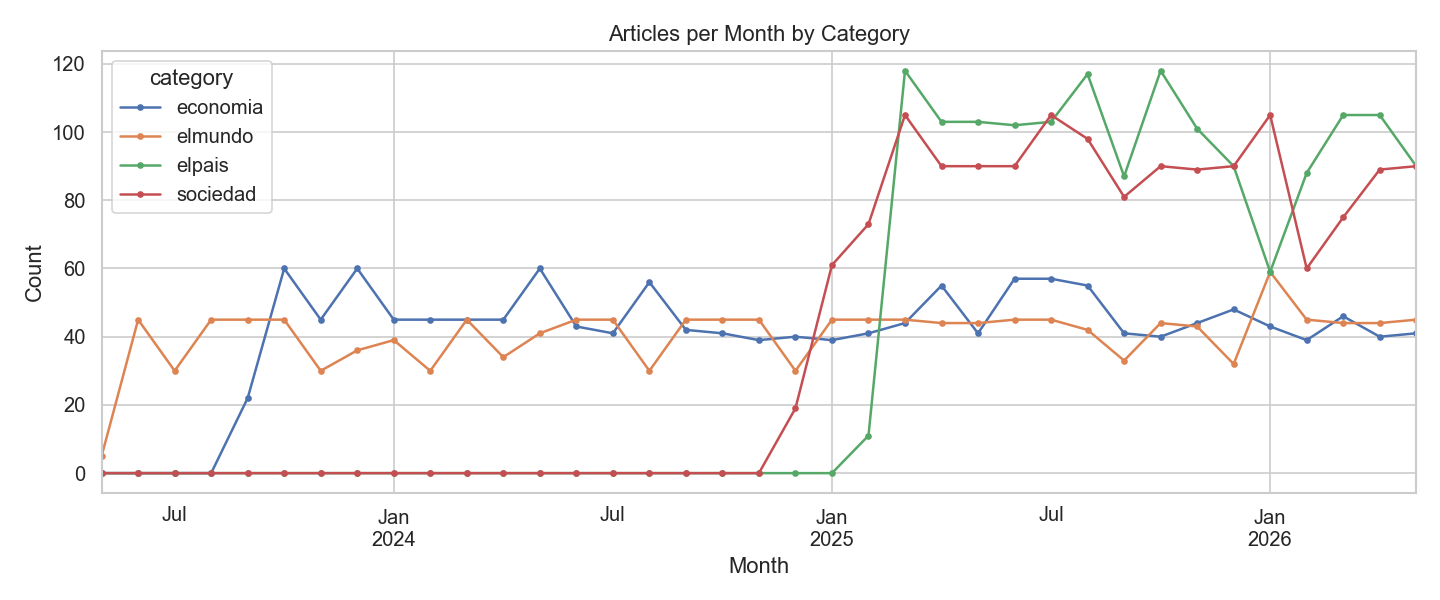
\includegraphics[width=0.95\textwidth]{articles_over_time.png}
\caption{Artículos por mes y sección. La cobertura temporal amplia mitiga el sesgo
de coyuntura.}
\label{fig:timeline}
\end{figure}

% ═════════════════════════════════════════════════════════════════════════════
\section{Extracción y preprocesamiento de texto}
% ═════════════════════════════════════════════════════════════════════════════
De cada artículo se extrajeron \emph{título}, \emph{bajada}, \emph{cuerpo},
\emph{fecha}, \emph{autor} y \emph{URL}. Las notas con cuerpo menor a 150
caracteres se descartan (zócalos, galerías, vivos). El texto se procesó con un
pipeline NLP configurable en español:
\begin{itemize}
  \item lectura en \textbf{UTF-8} (la consigna advierte sobre el \emph{encoding}: una
        lectura incorrecta rompe los acentos);
  \item eliminación de etiquetas HTML residuales y normalización Unicode (NFC);
  \item pasaje a minúsculas y eliminación de puntuación/números;
  \item remoción de \emph{stopwords} en español (lista de la cátedra);
  \item \emph{stemming} Snowball (opcional, evaluado).
\end{itemize}
La mediana resultante es de $\sim$\medTokens{} \emph{tokens} por artículo
(Figura~\ref{fig:tokens}), suficientemente larga para una clasificación léxica
robusta.

\begin{figure}[H]
\centering
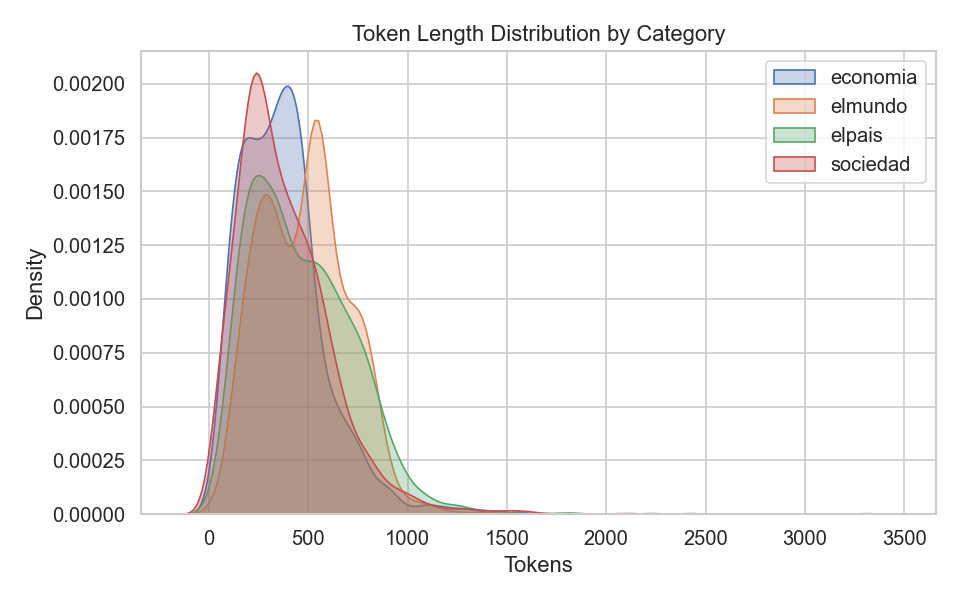
\includegraphics[width=0.7\textwidth]{token_distribution.png}
\caption{Distribución de longitud (tokens) por sección.}
\label{fig:tokens}
\end{figure}

% ═════════════════════════════════════════════════════════════════════════════
\section{Representaciones y modelos}
% ═════════════════════════════════════════════════════════════════════════════
Se evaluaron, como pide la consigna, un \textbf{baseline con Bag-of-Words/TF-IDF} y
al menos \textbf{una alternativa moderna} de representación (\emph{sentence
embeddings}). Todos los modelos se encapsularon en \texttt{Pipeline} de
\texttt{scikit-learn} para evitar fuga de información entre \emph{folds} (el
vectorizador se ajusta solo con el \emph{train} de cada \emph{fold}).

\begin{description}
  \item[BoW + Naive Bayes] \texttt{CountVectorizer} (unigramas) + Multinomial NB.
        Baseline explícito, rápido e interpretable.
  \item[BoW + Regresión Logística] \texttt{CountVectorizer} (1--2 gramas) + LR.
  \item[TF-IDF + Regresión Logística] ponderación TF-IDF \emph{sublinear} (1--2 gramas) + LR.
  \item[TF-IDF + LinearSVC] igual representación, clasificador de margen máximo
        lineal. \emph{Mejor modelo}.
  \item[Sentence embeddings + LR] \texttt{paraphrase-multilingual-MiniLM-L12-v2}
        (alternativa moderna). Se embebe \emph{título + bajada + inicio del cuerpo}
        para respetar el límite de 128 \emph{tokens} del modelo.
  \item[Ensambles] \emph{soft voting} y \emph{stacking} (meta-learner LR) sobre los
        modelos lineales.
\end{description}

% ═════════════════════════════════════════════════════════════════════════════
\section{Evaluación}
% ═════════════════════════════════════════════════════════════════════════════

\subsection{Validación cruzada (5-fold estratificado)}
Se reporta \emph{accuracy} y \textbf{Macro~F1} (esta última trata a las cuatro
clases por igual, lo importante con clases casi balanceadas pero donde interesa el
desempeño por sección). La Tabla~\ref{tab:cv} resume los resultados; la
Figura~\ref{fig:modelcomp} los compara visualmente.

\begin{table}[H]
\centering
\begin{tabular}{lcc}
\toprule
\textbf{Modelo} & \textbf{Accuracy} & \textbf{Macro F1} \\
\midrule
\textbf{TF-IDF + LinearSVC} & \textbf{0.904 $\pm$ 0.011} & \textbf{0.903 $\pm$ 0.011} \\
Ensamble (stacking) & 0.901 $\pm$ 0.009 & 0.901 $\pm$ 0.009 \\
TF-IDF + Reg. Logística & 0.900 $\pm$ 0.010 & 0.900 $\pm$ 0.010 \\
Ensamble (soft voting) & 0.890 $\pm$ 0.009 & 0.890 $\pm$ 0.009 \\
BoW + Reg. Logística & 0.885 $\pm$ 0.007 & 0.885 $\pm$ 0.007 \\
BoW + Naive Bayes & 0.883 $\pm$ 0.006 & 0.882 $\pm$ 0.006 \\
Sentence embeddings + LR & 0.818 $\pm$ 0.005 & 0.818 $\pm$ 0.005 \\
\bottomrule
\end{tabular}

\caption{Validación cruzada 5-fold estratificada. Media $\pm$ desvío entre folds.}
\label{tab:cv}
\end{table}

\begin{figure}[H]
\centering
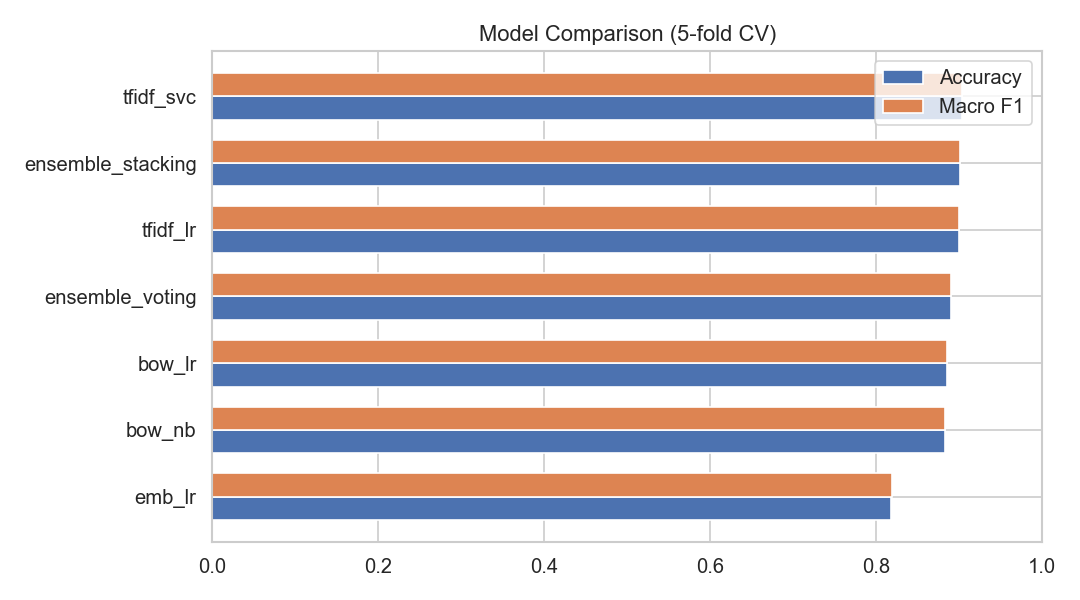
\includegraphics[width=0.85\textwidth]{model_comparison.png}
\caption{Comparación de modelos (Macro F1 y Accuracy en CV).}
\label{fig:modelcomp}
\end{figure}

\subsection{Matriz de confusión y clases difíciles}
La Figura~\ref{fig:cmcv} muestra la matriz de confusión promediada en CV del mejor
modelo (\emph{recall} por clase en la diagonal). Respondiendo a las preguntas
concretas de la consigna:
\begin{itemize}
  \item \textbf{¿Hay una clase más difícil?} Sí. \textbf{El País} es claramente la
        sección más difícil (\emph{recall} $\approx$85\,\%), seguida de
        \emph{Sociedad} ($\approx$87\,\%). En el otro extremo, \emph{El Mundo}
        ($\approx$95\,\%) y \emph{Economía} ($\approx$94\,\%) son las mejor
        separadas, gracias a su vocabulario característico (geopolítico:
        ``ONU'', ``Gaza'', ``Ucrania''; y económico: ``dólar'', ``inflación'',
        ``BCRA'').
  \item \textbf{¿Qué pares se confunden más?} El par más confundido es
        \textbf{El País $\leftrightarrow$ Sociedad} ($\approx$7\,\% en ambos
        sentidos, prácticamente \emph{simétrico}): ambas secciones tratan temas
        nacionales (política, salud, educación, derechos) con vocabulario solapado.
  \item \textbf{¿Hay confusión asimétrica?} Sí. El par \textbf{El País
        $\rightarrow$ Economía} ($\approx$5,4\,\%) supera al inverso
        \textbf{Economía $\rightarrow$ El País} ($\approx$3,6\,\%): una nota de
        política económica (``el Gobierno anunció medidas para contener la
        inflación'') tiene señales léxicas de ambas, pero el sesgo de error apunta
        \emph{de El País hacia Economía}, no al revés. Es decir, las notas
        políticas con jerga económica tienden a ser etiquetadas como Economía más
        que las notas económicas como política.
\end{itemize}

\begin{figure}[H]
\centering
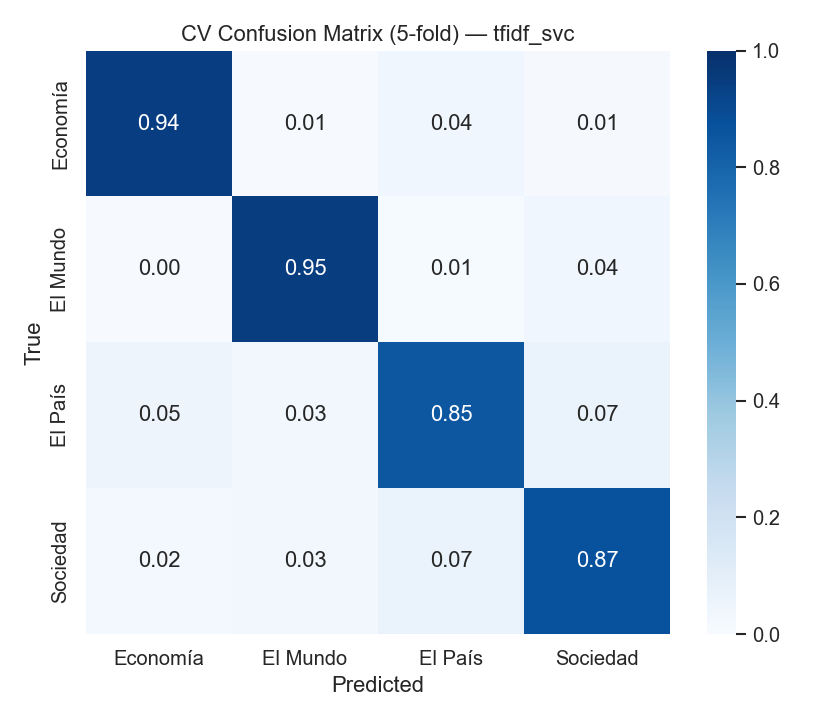
\includegraphics[width=0.62\textwidth]{cm_cv_tfidf_svc.png}
\caption{Matriz de confusión (CV 5-fold, normalizada por fila) del mejor modelo.}
\label{fig:cmcv}
\end{figure}

\subsection{Validación temporal (múltiples cortes)}
Se entrena con las notas anteriores a una fecha de corte y se evalúa con las
posteriores, simulando el uso real del modelo sobre noticias futuras. Como pide la
consigna (``idealmente, más de un corte temporal''), se evaluaron \textbf{tres
cortes} --- los últimos 3, 6 y 9 meses como conjunto de test --- para descartar que
un buen resultado sea un accidente de un período puntual.

\begin{table}[H]
\centering
\begin{tabular}{rlrrcc}
\toprule
\textbf{Corte} & \textbf{Fecha} & \textbf{Train} & \textbf{Test} & \textbf{Accuracy} & \textbf{Macro F1} \\
\midrule
3m & 2026-02-28 & 5185 & 814 & 0.853 & 0.858 \\
6m & 2025-11-29 & 4403 & 1596 & 0.848 & 0.853 \\
9m & 2025-08-29 & 3570 & 2429 & 0.846 & 0.849 \\
\midrule
\multicolumn{4}{r}{\textbf{Promedio}} & \textbf{0.849 $\pm$ 0.003} & \textbf{0.853 $\pm$ 0.004} \\
\bottomrule
\end{tabular}

\caption{Validación temporal en tres horizontes. El test es siempre posterior al
train. La estabilidad entre cortes confirma que el resultado no es casual.}
\label{tab:temporal}
\end{table}

\begin{figure}[H]
\centering
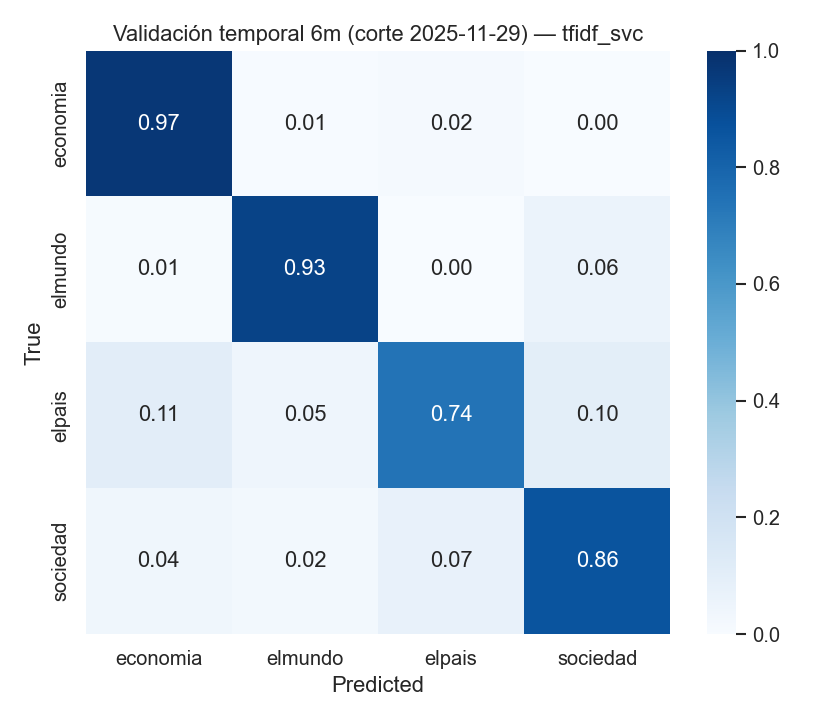
\includegraphics[width=0.62\textwidth]{cm_temporal_tfidf_svc_6m.png}
\caption{Matriz de confusión en validación temporal (corte de 6 meses).}
\label{fig:cmtemp}
\end{figure}

\subsection{¿Hay diferencia entre CV y validación temporal?}
La diferencia es \textbf{moderada pero muy estable}: el Macro~F1 cae de
\bestCVfone{} (CV) a \tempFmean{}~$\pm$~\tempFstd{} (temporal), unos 5 puntos. Lo
relevante es que los tres cortes dan valores casi idénticos (0,858 / 0,853 / 0,849)
pese a que el test crece de 814 a 2.429 noticias: el resultado \emph{no es un
accidente} de un período puntual. La explicación de la pequeña caída es doble: (i)
en CV el modelo puede ver vocabulario contemporáneo al test (mezcla de fechas),
mientras que en temporal entrena solo con el pasado; (ii) aun así el vocabulario que
define cada sección (jerga económica, organismos internacionales, actores políticos,
temas sociales) es \textbf{estable en el tiempo}, por lo que un modelo entrenado con
notas viejas sigue clasificando bien notas futuras. Una caída \emph{grande} habría
delatado sesgo temporal o \emph{overfitting} a la coyuntura del \emph{train}; una
caída chica y estable confirma que la solución generaliza.

% ═════════════════════════════════════════════════════════════════════════════
\section{Discusión de decisiones de diseño}
% ═════════════════════════════════════════════════════════════════════════════

\paragraph{Por qué TF-IDF supera a los embeddings.}
La tarea es de \emph{dominio léxico}, no de semántica profunda: las secciones se
distinguen por vocabulario específico (Economía: ``dólar'', ``inflación'',
``BCRA''; El Mundo: ``ONU'', ``Gaza'', ``Ucrania''). TF-IDF captura exactamente
esas señales discriminativas. Los \emph{embeddings} de MiniLM comprimen el texto en
un espacio semántico continuo donde términos de distinta sección quedan próximos
(p.\,ej.\ ``inflación'' y ``pobreza''), perdiendo poder discriminativo; además su
límite de 128 \emph{tokens} obliga a truncar artículos cuya mediana es de
$\sim$\medTokens{} \emph{tokens}. Por eso el \emph{baseline} clásico, bien
ajustado, resulta más fuerte que la alternativa moderna en esta tarea concreta.

\paragraph{Por qué el ensamble no mejora al mejor modelo individual.}
El \emph{stacking} reduce la varianza entre \emph{folds} pero no mejora la media:
los modelos base cometen \textbf{errores correlacionados} (todos confunden El País
con Sociedad y Economía), de modo que el meta-learner no encuentra señal
complementaria. El ensamble agrega valor cuando los errores son independientes, lo
que aquí no ocurre.

\paragraph{Generalización (no overfitting).}
Tres salvaguardas sostienen que el resultado generaliza: (i) toda la
vectorización vive dentro del \texttt{Pipeline} y se ajusta solo con el \emph{train}
de cada \emph{fold}, evitando fuga de información; (ii) la cobertura temporal amplia
del corpus evita el sesgo de coyuntura; y (iii) la validación temporal con múltiples
cortes confirma desempeño estable sobre noticias estrictamente futuras.

% ═════════════════════════════════════════════════════════════════════════════
\section{Conclusiones}
% ═════════════════════════════════════════════════════════════════════════════
Se obtuvo un clasificador de cuatro secciones con Macro~F1 de \bestCVfone{} (CV) y
$\sim$\tempFmean{} (temporal), usando una representación TF-IDF de \emph{n}-gramas
con un clasificador lineal de margen máximo. La alternativa moderna
(\emph{embeddings}) fue evaluada y resultó inferior por la naturaleza léxica de la
tarea, lo que constituye un hallazgo en sí mismo. La principal fuente de error es la
ambigüedad real entre \emph{El País} y \emph{Economía}, no una deficiencia del
modelo. La pequeña diferencia entre validación cruzada y temporal demuestra que la
solución generaliza a noticias futuras.

\appendix
% ═════════════════════════════════════════════════════════════════════════════
\section{Reproducibilidad}
% ═════════════════════════════════════════════════════════════════════════════
\begin{verbatim}
python scripts/run_scraper.py --articles-per-class 1500   # crawling (Arc API)
python scripts/parse_html.py                              # preprocesamiento NLP
python scripts/train.py                                   # entrenamiento + CV + temporal
python scripts/generate_report.py                         # reporte
python scripts/download_sample_html.py --per-class 12     # muestra HTML por sección
\end{verbatim}
Repositorio: \url{https://github.com/vic-ruiz/web_mining}

\end{document}
